% ------------------------------ title ----------------------------------
\title{Energy-Constrained UAV--UGV Replanning\\ under Dynamic Road Conditions}
\subtitle{End-Semester Evaluation: Method, Experiments and Results}
\author{Mayank Anand \and Sudhanshu \and Sujal}
\institute{Department of Information Technology\\
Indian Institute of Information Technology, Allahabad}
\date{}

\begin{document}

\begin{frame}\titlepage\end{frame}

\begin{frame}{1 \,Problem: A Team of UAVs and a UGV Charger}
\begin{columns}[T,onlytextwidth]
\begin{column}{0.52\textwidth}
\centering
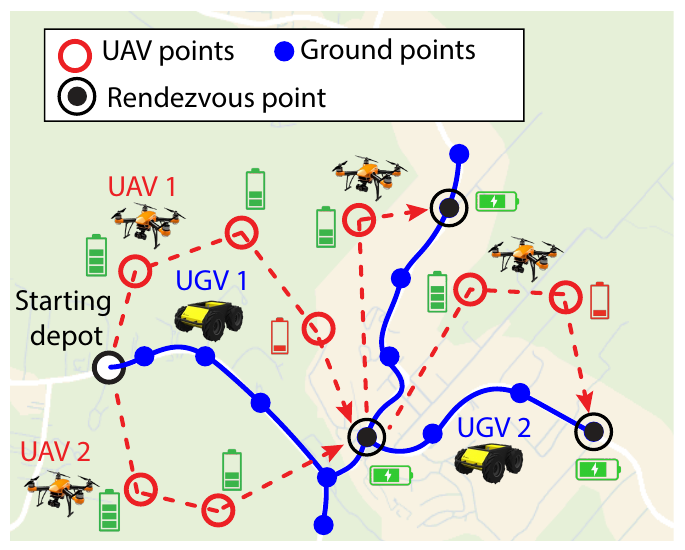
\includegraphics[width=\linewidth]{assets/base_fig1.png}\\[0.5mm]
{\tiny Illustration from Fig.~1 of~\cite{base}}
\end{column}
\begin{column}{0.46\textwidth}
\vspace{2mm}
\begin{tikzpicture}[node distance=5mm]
  \node[fteal, text width=4.6cm]  (a) {\textbf{UAVs} are fast but battery-limited\\(about 24 min of flight)};
  \node[fgray, text width=4.6cm, below=of a] (b) {\textbf{UGV} is slow, stays on roads,\\and charges one UAV at a time~\cite{base},~\cite{maini}};
  \node[fnavy, text width=4.6cm, below=of b] (c) {\textbf{Goal:} visit every task point\\as fast as possible};
  \draw[ar] (a) -- (b); \draw[ar] (b) -- (c);
\end{tikzpicture}
\end{column}
\end{columns}
\end{frame}

\begin{frame}{1 \,Intuition: One Sortie, Step by Step}
\centering
\begin{tikzpicture}
  \node[fb] (n1) at (0,2.2) {Take off\\ full battery};
  \node[fb] (n2) at (3.0,2.2) {Visit task points\\ (battery check)};
  \node[dia, text width=1.5cm] (d1) at (6.3,2.2) {Battery low\\or all done?};
  \node[fb] (n3) at (9.6,2.2) {Fly to rendezvous,\\ land on UGV};
  \node[famber] (n4) at (12.6,2.2) {\textbf{Hover} until\\ UGV arrives};
  \node[fb] (n5) at (12.6,0) {Recharge\\ $T_R=15$ min};
  \node[dia, text width=1.4cm] (d2) at (9.3,0) {Tasks\\left?};
  \node[fnavy] (n6) at (5.9,0) {Mission done};
  \draw[ar] (n1)--(n2); \draw[ar] (n2)--(d1);
  \draw[ar] (d1)-- node[above,lab]{yes} (n3);
  \draw[ar] (n3)--(n4); \draw[ar] (n4)--(n5); \draw[ar] (n5)--(d2);
  \draw[ar] (d2)-- node[above,lab]{no} (n6);
  \draw[ar] (d1.north) -- ++(0,0.65) -| node[pos=0.25,above,lab]{no: keep visiting} (n2.north);
  \draw[ar] (d2.south) -- ++(0,-0.6) -| node[pos=0.25,below,lab]{yes: next sortie} (n1.south);
\end{tikzpicture}\\[3mm]
{\small The UGV is the bottleneck: it drives at 4.5\,m/s, the UAV flies at 10\,m/s \cite{base}.}
\end{frame}

\begin{frame}{1 \,Why It Gets Harder: Roads Change During the Mission}
\centering
\begin{tikzpicture}
  \node[fred]   (a) at (0,0)    {Road blocked\\ or slowed};
  \node[fgray]  (b) at (2.9,0)  {UGV detours,\\ arrives late};
  \node[famber] (c) at (5.8,0)  {UAV hovers\\ longer};
  \node[famber] (d) at (8.7,0)  {Extra\\ energy used};
  \node[fred]   (e) at (11.6,0) {Over budget or\\ missed recharge};
  \foreach \x/\y in {a/b,b/c,c/d,d/e} \draw[arr] (\x) -- (\y);
\end{tikzpicture}\\[7mm]
\begin{tikzpicture}[scale=1.0, font=\scriptsize]
  \node[circle, fill=Midnight, inner sep=1.6pt, label=left:UGV] (A) at (0,0) {};
  \node[circle, fill=Teal, inner sep=1.6pt, label=right:rendezvous] (B) at (3.2,0) {};
  \node[circle, fill=gray, inner sep=1pt] (C) at (0,1.6) {};
  \node[circle, fill=gray, inner sep=1pt] (D) at (3.2,1.6) {};
  \draw[red!70!black, very thick] (A)--(B);
  \node[red!70!black, font=\large] at (1.6,0) {$\times$};
  \node[below, text=Muted] at (1.6,-0.15) {direct road: 2.7 km, 10 min};
  \draw[gray, thick, dashed] (A)--(C)--(D)--(B);
  \node[above, text=Muted] at (1.6,1.65) {detour: 8.1 km, 30 min};
  \node[align=left, right] at (4.8,0.8) {\textbf{Hand-checked case:}\\the UAV waits 19 more minutes,\\costing 262\,kJ of hover energy.};
\end{tikzpicture}
\end{frame}

\begin{frame}{1 \,Problem Statement}
\centering
\begin{tikzpicture}
  \node[fgray, text width=3.1cm] (in) at (0,0.9) {\textbf{Inputs}\\[0.5mm] task points, fleet,\\road graph $G_t$, budget $B$};
  \node[fnavy, text width=2.6cm, minimum height=1.6cm] (pl) at (4.6,0.9) {\textbf{Planner}\\(learned policy)};
  \node[fteal, text width=3.7cm] (out) at (9.4,0.9) {\textbf{Outputs}\\[0.5mm] UAV sorties, UGV routes,\\rendezvous schedule};
  \draw[ar] (in) -- (pl); \draw[ar] (pl) -- (out);
  \node[famber, text width=3.4cm] (ev) at (4.6,-1.05) {Road events\\(blocked / slow)};
  \draw[arr] (ev) -- (pl);
  \draw[ar, dashed] (out.south) |- node[pos=0.7,below,lab]{replan if the plan becomes infeasible} (ev.east);
\end{tikzpicture}\\[2mm]
\begin{block}{Formulation}
\centering
$\displaystyle \min\; T \quad\text{s.t.}\quad E\le B=\beta B_0,\;\; \beta\in\{0.7,0.8,0.9,1.0\}$
\end{block}
\vspace{-1mm}
\begin{center}
\chip{Teal}{every task visited}\;\chip{Teal}{sortie within battery $F_a$}\;\chip{Teal}{rendezvous on a reachable road node}\;\chip{Teal}{one UAV per UGV at a time}
\end{center}
{\scriptsize Energy $E=\sum\big(P_{\text{fly}}t_{\text{fly}}+P_{\text{hover}}t_{\text{wait}}\big)$ with the power model of~\cite{base},~\cite{hurwitz}.}
\end{frame}

\begin{frame}{2 \,Literature: How the Field Got Here}
\centering
\begin{tikzpicture}
  \foreach \y/\t in {3.5/Optimisation, 1.9/Learning-based routing, 0.3/Energy and uncertainty}
    \node[anchor=west, font=\scriptsize\bfseries, text=Midnight] at (-0.7,\y+0.78) {\t};
  \node[fgray, text width=3.1cm] (m)  at (1.3,3.5)  {Maini et al. 2019~\cite{maini}\\ MILP + heuristics,\\ 1 UAV + 1 UGV};
  \node[fgray, text width=3.1cm] (mr) at (6.4,3.5)  {Mondal et al. 2023~\cite{mrs}\\ bilevel planning,\\ large coverage};
  \node[fgray, text width=3.1cm] (f)  at (6.4,1.9)  {Fan et al. 2023~\cite{fan}\\ DRL, 1 UAV,\\ many chargers};
  \node[fteal, text width=3.2cm] (b)  at (11.3,1.9) {\textbf{Mondal et al. 2025~\cite{base}}\\ Transformer DRL,\\ multi UAV--UGV};
  \node[fgray, text width=3.1cm] (s)  at (1.3,0.3)  {Shi et al. 2022~\cite{shi}\\ chance-constrained\\ MDP rendezvous};
  \node[fgray, text width=3.1cm] (l)  at (6.4,0.3)  {Lin et al. 2022~\cite{lin}\\ robust surveillance,\\ charging stations};
  \node[fgray, text width=3.2cm] (r)  at (11.3,0.3) {Mondal et al. 2025~\cite{icra}\\ risk-aware attention RL,\\ uncertain fuel};
  \draw[ar] (m) -- (mr); \draw[ar] (f) -- (b); \draw[ar] (mr.south east) -- (b.north west);
  \draw[ar] (s) -- (l); \draw[ar] (l) -- (r);
\end{tikzpicture}\\[1mm]
{\scriptsize Left to right = later work. The base paper \cite{base} compares against the bilevel line~\cite{mrs} and extends the DRL line~\cite{fan}.}
\end{frame}

\begin{frame}{2 \,Research Gap}
\centering\scriptsize
\renewcommand{\arraystretch}{1.3}
\begin{tabular}{@{}P{3.4cm}cccc@{}}
\toprule
Work & \makecell{Learned\\policy} & \makecell{Multi\\UAV--UGV} & \makecell{Mission energy\\budget} & \makecell{Roads change\\during mission}\\
\midrule
Mondal et al.~\cite{base} (base) & \cmark & \cmark & \xmark & \xmark\\
Mondal et al.~\cite{icra} & \cmark & \pmark & \pmark (fuel risk) & \xmark\\
Shi et al.~\cite{shi} & \xmark & \xmark & \pmark (fuel risk) & \xmark\\
Lin et al.~\cite{lin} & \xmark & \cmark & \pmark (feasibility) & \pmark (obstacles)\\
\midrule
\textbf{This work} & \cmark & \cmark & \cmark & \cmark\\
\bottomrule
\end{tabular}\\[3mm]
{\tiny \cmark\ addressed \quad \pmark\ partial \quad \xmark\ not addressed}\\[3mm]
\begin{tikzpicture}
  \node[fnavy, text width=11.5cm] {No reviewed work combines a learned multi-UAV--UGV policy, a mission energy budget, and roads that change during the mission.};
\end{tikzpicture}
\end{frame}

\begin{frame}{2 \,From the Gap to Our Questions}
\centering
\begin{tikzpicture}[node distance=3mm]
  \node[fnavy, text width=2.6cm, minimum height=3.6cm] (g) at (0,0) {Gap:\\ energy budget\\ + changing roads};
  \node[fteal, text width=4.6cm] (q1) at (4.4,1.8)  {\textbf{RQ1} Time--energy trade-off?};
  \node[fteal, text width=4.6cm] (q2) at (4.4,0.6)  {\textbf{RQ2} Stay within a budget?};
  \node[fteal, text width=4.6cm] (q3) at (4.4,-0.6) {\textbf{RQ3} Effect of blockages?};
  \node[fteal, text width=4.6cm] (q4) at (4.4,-1.8) {\textbf{RQ4} Event-triggered vs periodic replanning?};
  \node[famber, text width=4.4cm] (h1) at (10.2,1.8)  {H1: energy falls, time barely rises};
  \node[famber, text width=4.4cm] (h2) at (10.2,0.6)  {H2: constrained beats fixed penalty};
  \node[famber, text width=4.4cm] (h3) at (10.2,-0.6) {H3: more disruption, more energy};
  \node[famber, text width=4.4cm] (h4) at (10.2,-1.8) {H4: same reliability, fewer replans};
  \foreach \i in {1,2,3,4} {\draw[ar] (g.east) -- (q\i.west); \draw[ar] (q\i) -- (h\i);}
\end{tikzpicture}
\end{frame}

\begin{frame}{3 \,Before Mid-Sem: What We Did}
\centering
\begin{tikzpicture}
  \node[fgray, text width=1.9cm] (a) at (0,1.2)   {Studied the base paper~\cite{base}};
  \node[fgray, text width=1.9cm] (b) at (2.4,1.2) {Found its limits};
  \node[fgray, text width=1.9cm] (c) at (4.8,1.2) {Formalised $\min T$ s.t. $E\le B$};
  \node[fgray, text width=1.9cm] (d) at (7.2,1.2) {Road, energy and budget models};
  \node[fgray, text width=1.9cm] (e) at (9.6,1.2) {Candidate methods A and B};
  \node[fgray, text width=1.9cm] (f) at (12.0,1.2){Replanning design};
  \foreach \x/\y in {a/b,b/c,c/d,d/e,e/f} \draw[ar] (\x) -- (\y);
  \node[fgray, text width=5.6cm] (g) at (3.4,-0.5) {Experimental plan: policies P0--P4, stages A, B, C};
  \node[fgray, text width=5.6cm] (h) at (9.6,-0.5) {Gazebo testbed started: desert terrain + 4-wheel UGV~\cite{gazebo}};
  \draw[ar] (c.south) -- (g.north); \draw[ar] (f.south) -- (h.north);
\end{tikzpicture}\\[3mm]
{\small A proposal and design phase: \textbf{no learned results yet}.}
\end{frame}

\begin{frame}{3 \,Before Mid-Sem: The Proposed Framework}
\centering
\begin{tikzpicture}
  \node[fgray, text width=1.9cm]  (i) at (0,2.0)    {Instance\\ $(x_i,y_i,b_i)$};
  \node[fgray, text width=2.0cm]  (e) at (2.6,2.0)  {Encoder\\ (unchanged)};
  \node[fteal, text width=2.5cm]  (d) at (5.5,2.0)  {Route decoder\\ {\scriptsize (+ budget input in B)}};
  \node[fgray, text width=2.7cm]  (a) at (8.7,2.0)  {Greedy assignment (frozen)};
  \node[fgray, text width=2.0cm]  (s) at (11.8,2.0) {Simulator\\ $T$, $E$};
  \node[fteal, text width=2.2cm]  (r) at (11.8,0.2) {Road layer\\ events on $G_t$};
  \node[fteal, text width=2.5cm]  (c) at (8.7,0.2)  {Check reach and time};
  \node[fteal, text width=2.3cm]  (m) at (5.5,0.2)  {Updated action masks};
  \draw[ar] (i)--(e); \draw[ar] (e)--(d); \draw[ar] (d)--(a); \draw[ar] (a)--(s);
  \draw[ar] (s)--(r); \draw[ar] (r)--(c); \draw[ar] (c)--(m); \draw[ar] (m)--node[right,lab]{replan} (d);
  \node[famber, text width=5.6cm] (A) at (2.9,-1.5) {\textbf{A} Lagrangian: $T+\lambda\max(0,E-B)$};
  \node[famber, text width=6.0cm] (B) at (9.3,-1.5) {\textbf{B} Budget-conditioned: input $b_t=(B-E_t)/B$};
\end{tikzpicture}\\[1mm]
{\scriptsize \colorbox{gray!13}{\strut kept from base~\cite{base}}\;\colorbox{Teal!14}{\strut new}\;\colorbox{Amber!24}{\strut candidate method}}
\end{frame}

\begin{frame}{4 \,Challenges and Limits Before Mid-Sem $\rightarrow$ What We Did About Them}
\centering
\begin{tikzpicture}[font=\scriptsize]
  \foreach \i/\l/\r in {
    0/{No implementation, only a plan}/{Simulator + learned policy, 35 tests},
    1/{Base method not verified}/{Compared with \cite{base} on its own map},
    2/{Unknown details: $T_R$, road map}/{Confirmed from the authors' code~\cite{code}},
    3/{Only tree roads: no detours}/{Maps with loops: ring, border, district},
    4/{Energy gain only illustrated}/{Measured: 4 maps $\times$ 3 seeds $\times$ 100 instances},
    5/{Physics not validated}/{3D replay and Gazebo replay of the plans}} {
    \node[fred, text width=4.6cm] (l\i) at (0,-\i*1.05) {\l};
    \ifnum\i=5 \node[famber, text width=5.2cm] (r\i) at (8.9,-\i*1.05) {\r};
    \else \node[fteal, text width=5.2cm] (r\i) at (8.9,-\i*1.05) {\r}; \fi
    \draw[ar] (l\i) -- (r\i);}
  \node[lab] at (0,0.7) {before mid-sem}; \node[lab] at (8.9,0.7) {after mid-sem};
\end{tikzpicture}
\end{frame}

\begin{frame}{5 \,Step 1: Reproduce the Base on Its Own Map}
\begin{columns}[T,onlytextwidth]
\begin{column}{0.58\textwidth}
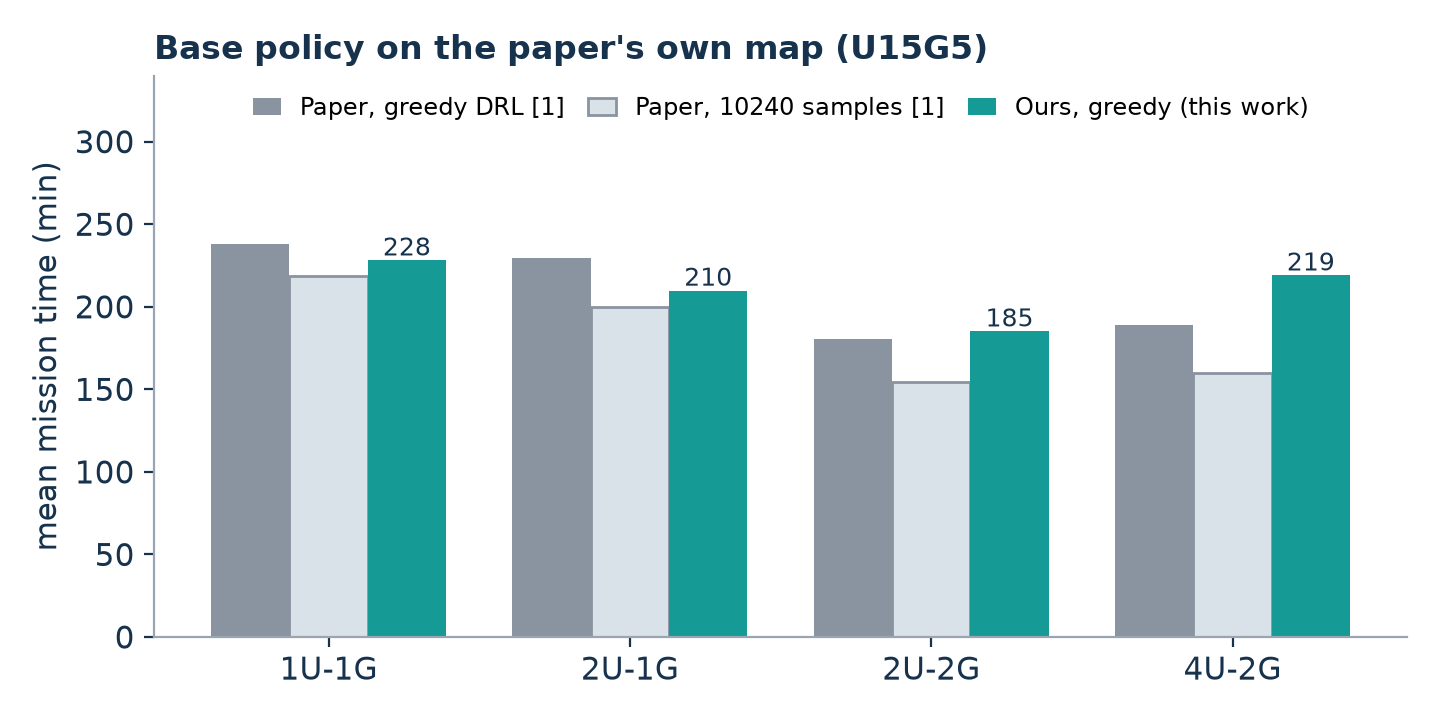
\includegraphics[width=\linewidth]{assets/fig_tableI.png}
\end{column}
\begin{column}{0.40\textwidth}
\vspace{1mm}
\begin{tikzpicture}[node distance=3.5mm]
  \node[fgray, text width=3.7cm] (a) {Authors' code~\cite{code}};
  \node[fteal, text width=3.7cm, below=of a] (b) {28 road points, 3 chains\\ \cmark};
  \node[fteal, text width=3.7cm, below=of b] (c) {$T_R=900$\,s, wait rules\\ \cmark};
  \node[fnavy, text width=3.7cm, below=of c] (d) {Our simulator and policy};
  \draw[ar] (a)--(b); \draw[ar] (b)--(c); \draw[ar] (c)--(d);
\end{tikzpicture}
\end{column}
\end{columns}
{\scriptsize Within about 10\% of \cite{base} for three of four teams; 4U-2G is still 9 to 14\% slower even after 3000 training steps (3 seeds).}
\end{frame}

\begin{frame}{5 \,Step 2: Event-Triggered Replanning}
\begin{columns}[T,onlytextwidth]
\begin{column}{0.62\textwidth}
\centering
\begin{tikzpicture}
  \node[famber, text width=3.0cm] (a) at (0,3.3) {Road event observed};
  \node[fb, text width=3.0cm] (b) at (0,2.35) {Update the road graph};
  \node[fb, text width=3.0cm] (c) at (0,1.4) {Re-time the remaining plan};
  \node[dia, text width=2.0cm, minimum height=1.1cm] (d) at (0,0.1) {Plan still\\valid?};
  \node[fteal, text width=2.6cm] (e) at (4.3,0.1) {Replan remaining tasks (keep completed route)};
  \node[fgray, text width=2.6cm] (f) at (0,-1.4) {Keep the plan};
  \node[fred, text width=2.7cm] (g) at (4.3,1.6) {Invalid if: unreachable, over budget, or UAV waits 5 min longer};
  \draw[ar] (a)--(b); \draw[ar] (b)--(c); \draw[ar] (c)--(d);
  \draw[arg] (d.east) -- node[above,lab]{no} (e.west);
  \draw[ar] (d.south) -- node[right,lab]{yes} (f.north);
  \draw[ar, dashed] (g.south) -- (e.north);
\end{tikzpicture}
\end{column}
\begin{column}{0.35\textwidth}
\vspace{2mm}\small
\begin{tabular}{@{}P{1.9cm}P{2.2cm}@{}}
\toprule
\textbf{Controller} & \textbf{Replans when}\\
\midrule
Open-loop & never\\[1mm]
Periodic & every recharge\\[1mm]
\textbf{Event-triggered} & only if the plan breaks\\
\bottomrule
\end{tabular}\\[3mm]
{\footnotesize A UAV with a stranded rendezvous may divert on its remaining battery.}
\end{column}
\end{columns}
\end{frame}

\begin{frame}{5 \,Step 3: Learning the Policies}
\centering
\begin{tikzpicture}
  \node[fgray, text width=2.1cm] (a) at (-0.3,0.9)    {Clone the rule policy (imitation)};
  \node[fteal, text width=2.4cm] (b) at (2.7,0.9) {REINFORCE on time: \textbf{P0}, the base};
  \draw[ar] (a)--(b);
  \node[fb, text width=3.2cm]    (v1) at (6.9,2.5) {P0+ control: same extra training};
  \node[fb, text width=3.2cm]    (v2) at (6.9,1.5) {P2: fixed penalty $T+\alpha E$};
  \node[famber, text width=3.2cm] (v3) at (6.9,0.5) {P3 (A): Lagrangian};
  \node[famber, text width=3.2cm] (v4) at (6.9,-0.5) {P4 (B): budget input};
  \foreach \p in {v1,v2,v3,v4} \draw[ar] (b.east) -- (\p.west);
  \node[fteal, text width=3.2cm] (p1) at (11.2,0.9) {P1 (at inference): sample $N$ routes, keep the fastest with $E\le B$};
  \draw[ar, dashed] (b.south) -- ++(0,-1.3) -| (p1.south);
\end{tikzpicture}\\[2mm]
{\small Transformer policy of~\cite{base} (attention model~\cite{kool}) trained with REINFORCE~\cite{williams}; all variants start from the same P0.}
\end{frame}

\begin{frame}{5 \,Step 4: Experimental Design}
\centering
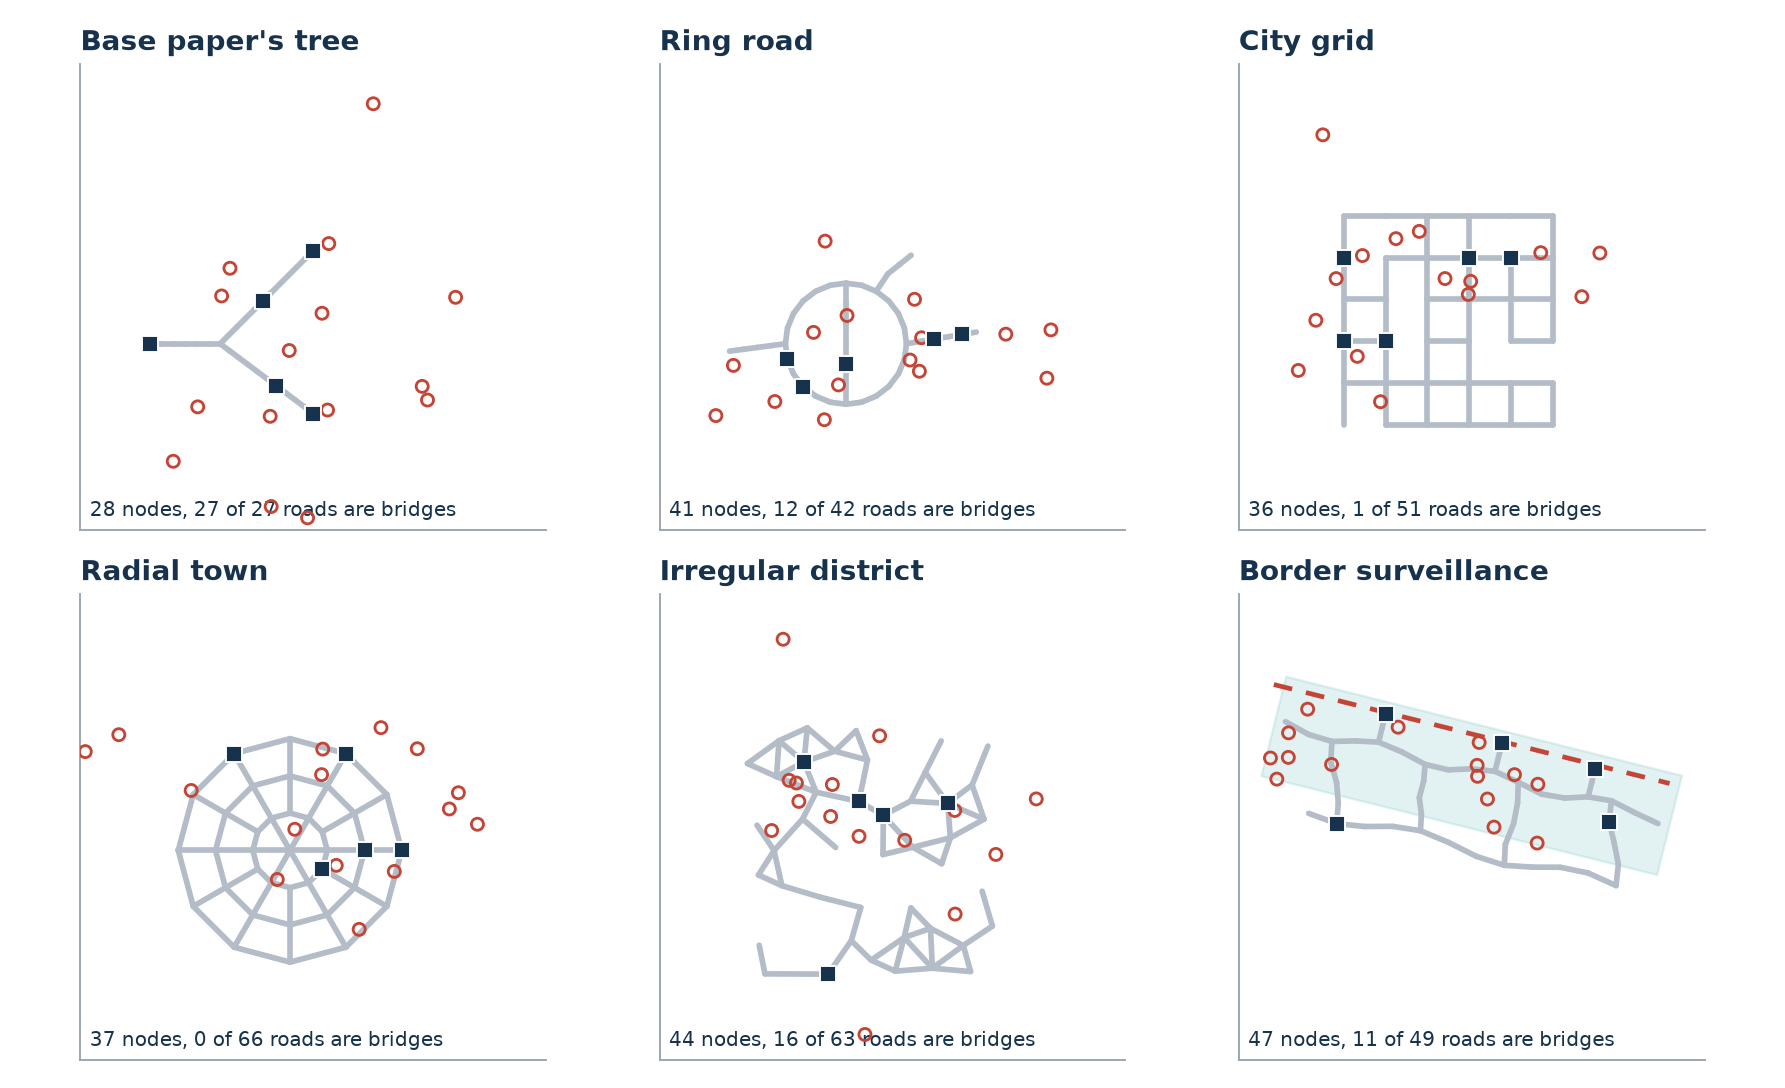
\includegraphics[height=0.56\textheight]{assets/fig_maps.png}\\[0.5mm]
{\scriptsize Road maps used (squares = ground points, circles = aerial tasks; shaded strip and dashed line = border).}\\[1.5mm]
\chip{Teal}{4 maps, 4 team sizes}\;\chip{Teal}{3 training seeds}\;\chip{Teal}{100 test instances}\;\chip{Teal}{18 road events}\;\chip{Amber}{Kaggle CPU, about 3 h per map}\\[1.5mm]
{\scriptsize 18 events = \{blocked, slow\} $\times$ \{low, medium, high\} $\times$ \{early, middle, late\}}
\end{frame}

\begin{frame}{6 \,Result 1: Road Events Really Hurt}
\centering
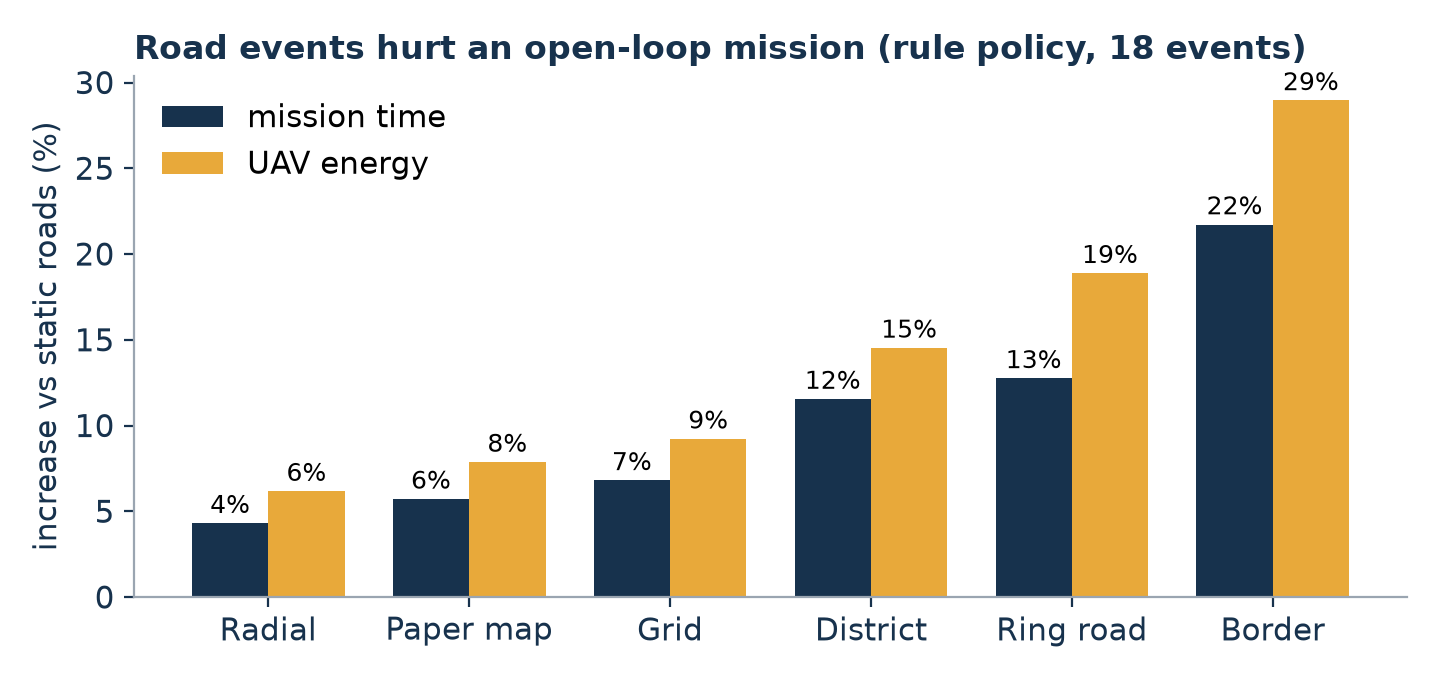
\includegraphics[width=0.78\linewidth]{assets/fig_damage.png}\\[1mm]
{\small The border-surveillance map is the most sensitive; the radial map, full of detours, the least.}
\end{frame}

\begin{frame}{6 \,Result 2: Replanning Recovers Time and Energy, With Few Replans}
\centering
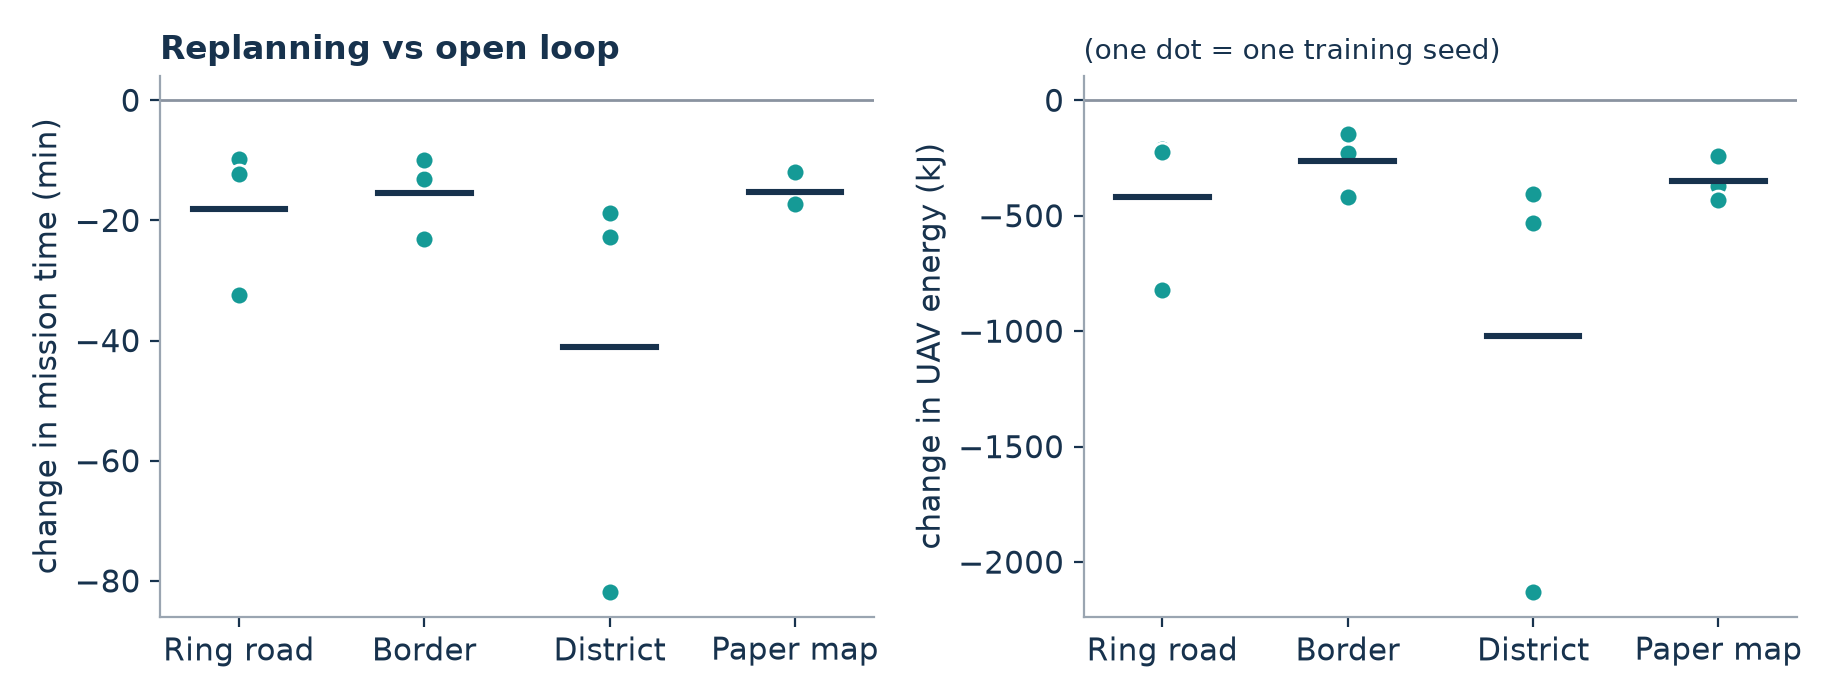
\includegraphics[width=0.88\linewidth]{assets/fig_replan_gain.png}\\[0.5mm]
\begin{tikzpicture}\node[fteal, text width=12.2cm]{Better than open loop in \textbf{all 12} map--seed combinations (15 to 41\,min, 260 to 1000\,kJ saved). Event-triggered replanning matches periodic replanning (within 0.3\,min) with \textbf{1 to 3 fewer replans} per mission.};\end{tikzpicture}
\end{frame}

\begin{frame}{6 \,Result 3: Why the Energy Methods Have So Little to Gain}
\centering
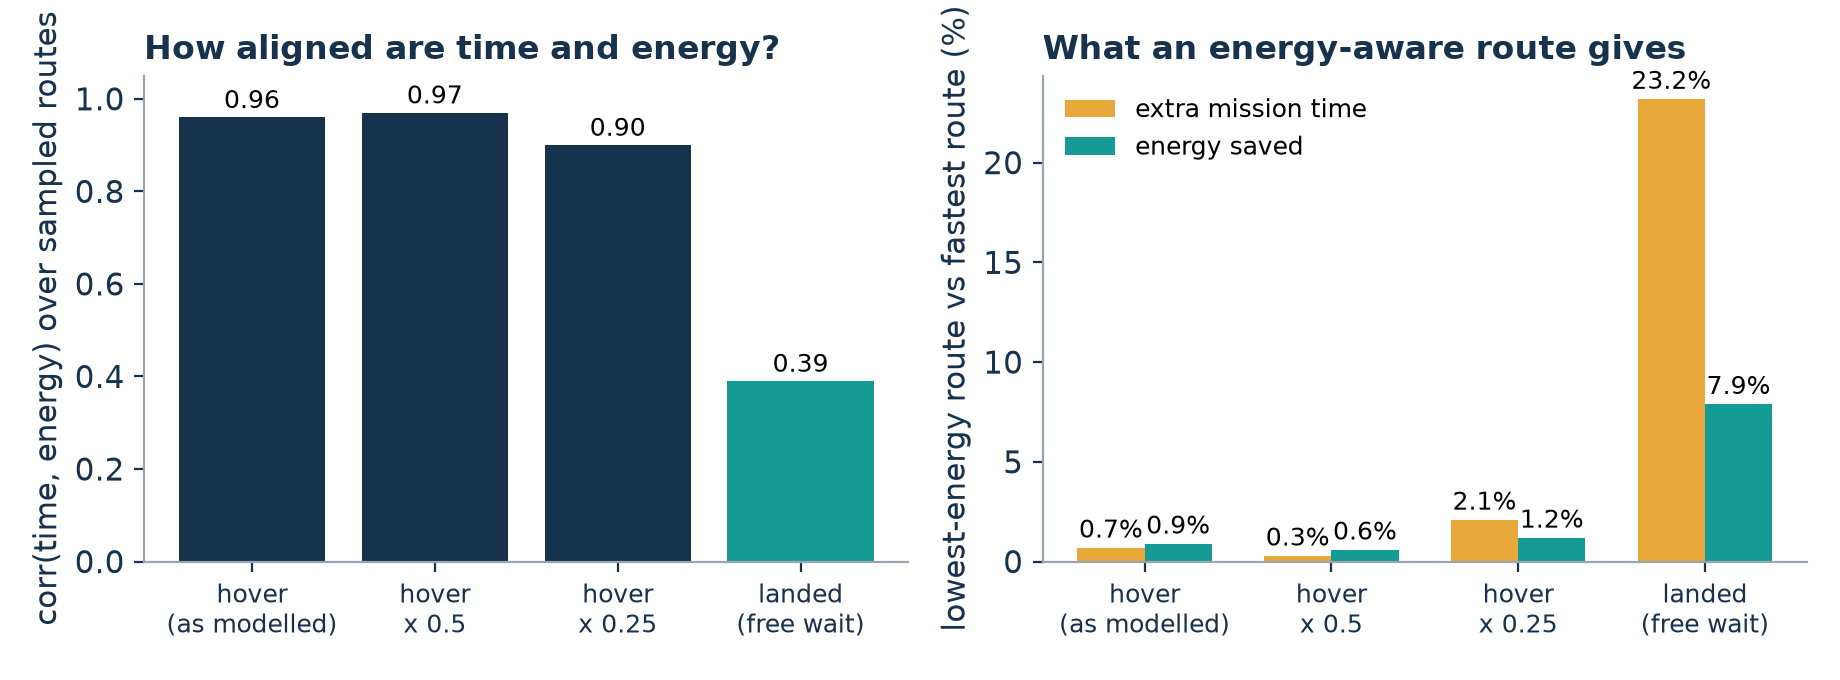
\includegraphics[width=0.88\linewidth]{assets/fig_tradeoff.png}\\[1mm]
\begin{tikzpicture}[font=\scriptsize]
  \node[famber, text width=2.5cm] (a) at (0,0)  {Hover waiting is about half of $E$};
  \node[fgray,  text width=2.5cm] (b) at (3.4,0) {Faster routes wait less};
  \node[fgray,  text width=2.5cm] (c) at (6.8,0) {Fastest $\approx$ lowest-energy route};
  \node[fred,   text width=3.0cm] (d) at (10.4,0){No trade-off to learn (H1)};
  \foreach \x/\y in {a/b,b/c,c/d} \draw[ar] (\x)--(\y);
\end{tikzpicture}
\end{frame}

\begin{frame}{6 \,Result 4: A Lever That Realises the Idea}
\centering
\begin{tikzpicture}[x=0.118cm, y=1cm]
  \node[anchor=east, font=\scriptsize\bfseries] at (-1,3.45) {Before};
  \fill[Midnight] (0,3.2) rectangle (24,3.7); \fill[Amber] (24,3.2) rectangle (40,3.7); \fill[gray!45] (40,3.2) rectangle (55,3.7);
  \node[font=\tiny, text=white] at (12,3.45) {flying}; \node[font=\tiny] at (32,3.45) {hovering}; \node[font=\tiny] at (47.5,3.45) {charging};
  \node[anchor=east, font=\scriptsize\bfseries] at (-1,1.85) {After};
  \fill[gray!25] (0,1.6) rectangle (16,2.1); \fill[Midnight] (16,1.6) rectangle (40,2.1); \fill[gray!45] (40,1.6) rectangle (55,2.1);
  \node[font=\tiny] at (8,1.85) {waits on the ground}; \node[font=\tiny, text=white] at (28,1.85) {flying}; \node[font=\tiny] at (47.5,1.85) {charging};
  \fill[Teal!70] (0,0.2) rectangle (40,0.7); \fill[gray!45] (40,0.2) rectangle (55,0.7);
  \node[anchor=east, font=\scriptsize\bfseries] at (-1,0.45) {UGV};
  \node[font=\tiny] at (20,0.45) {driving to the rendezvous}; \node[font=\tiny] at (47.5,0.45) {charging};
  \draw[dashed, Midnight!60] (40,0.1) -- (40,3.9);
  \node[lab] at (40,4.1) {UGV arrives: same moment in both};
  \draw[->] (0,-0.2) -- (60,-0.2); \node[font=\tiny, below] at (30,-0.2) {mission time};
\end{tikzpicture}\\[4mm]
\begin{tikzpicture}
  \node[famber, text width=3.2cm] (a) at (0,0)    {UAV expects to arrive before the UGV};
  \node[fteal,  text width=3.2cm] (b) at (3.9,0)  {Delay take-off by the expected wait};
  \node[fgray,  text width=3.2cm] (c) at (7.8,0)  {Arrives as the UGV arrives: no hovering};
  \node[fnavy,  text width=3.2cm] (d) at (11.7,0) {Same mission time, far less energy};
  \foreach \x/\y in {a/b,b/c,c/d} \draw[ar] (\x)--(\y);
\end{tikzpicture}\\[2mm]
{\small Assumption: a UAV can wait on the ground at its charging point for free, and a delay is predicted from the road state it knows.}
\end{frame}

\begin{frame}{6 \,Result 5: Sampling and Just-in-Time Together}
\centering
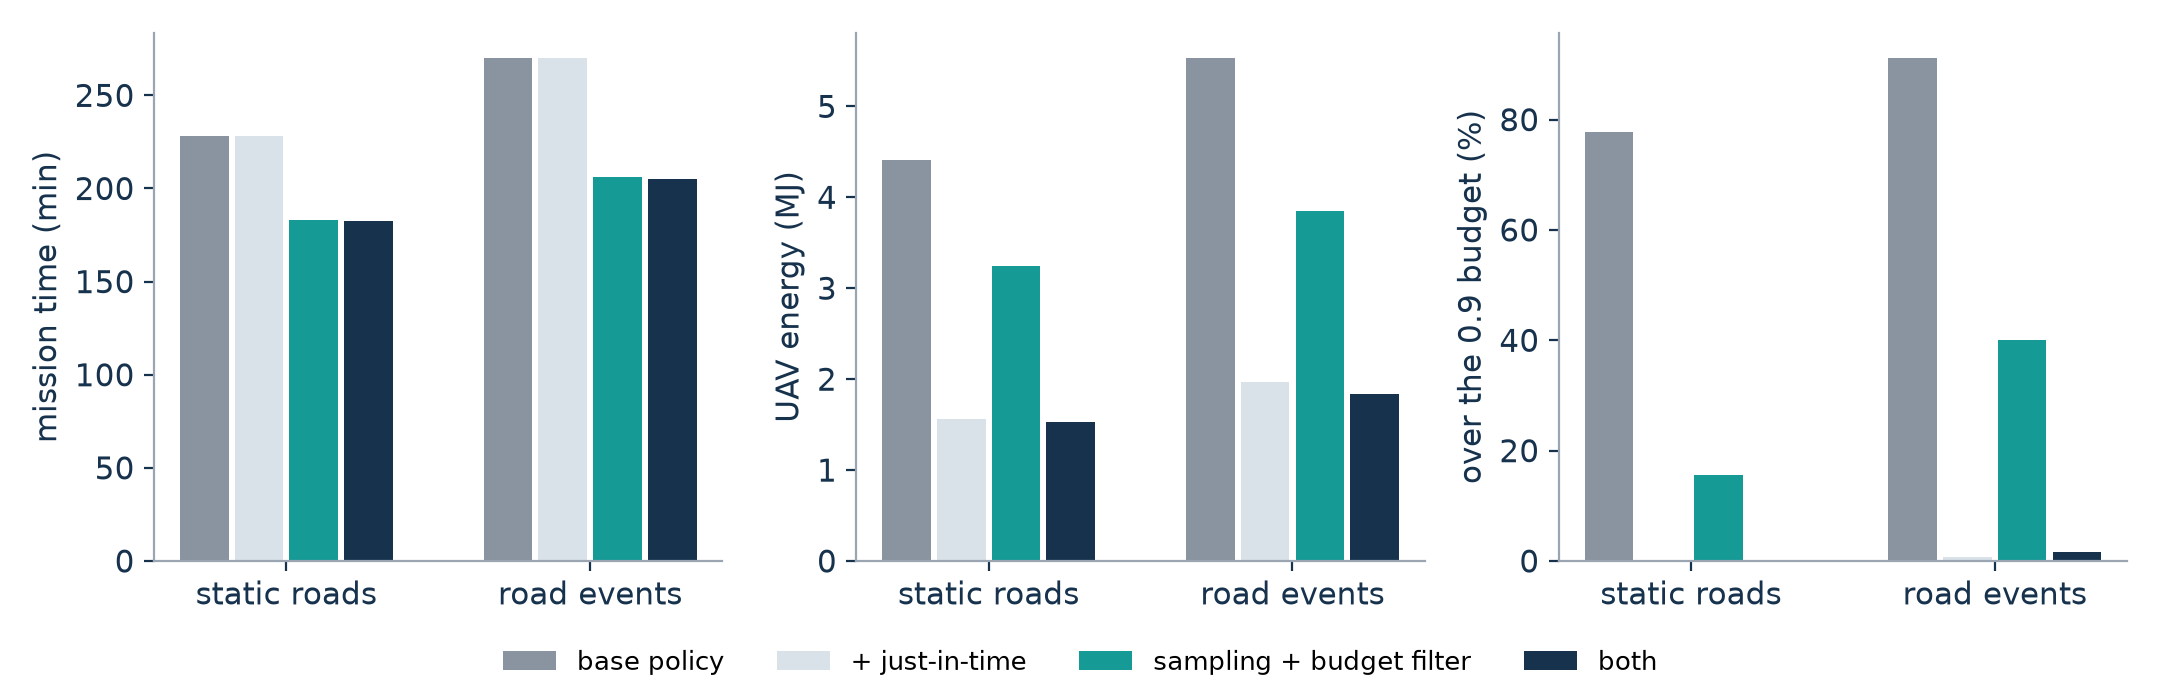
\includegraphics[width=0.97\linewidth]{assets/fig_headline.png}\\[0.5mm]
{\small 4 maps $\times$ 3 seeds, 2U-1G. Sampling cuts time by 20\%, just-in-time departure cuts energy by 65\%; together the gains add up and the budget is met (0\% violations, 2\% with events).}
\end{frame}

\begin{frame}{6 \,Result 6: Baselines and Sampled Decoding (Paper's Map)}
\centering
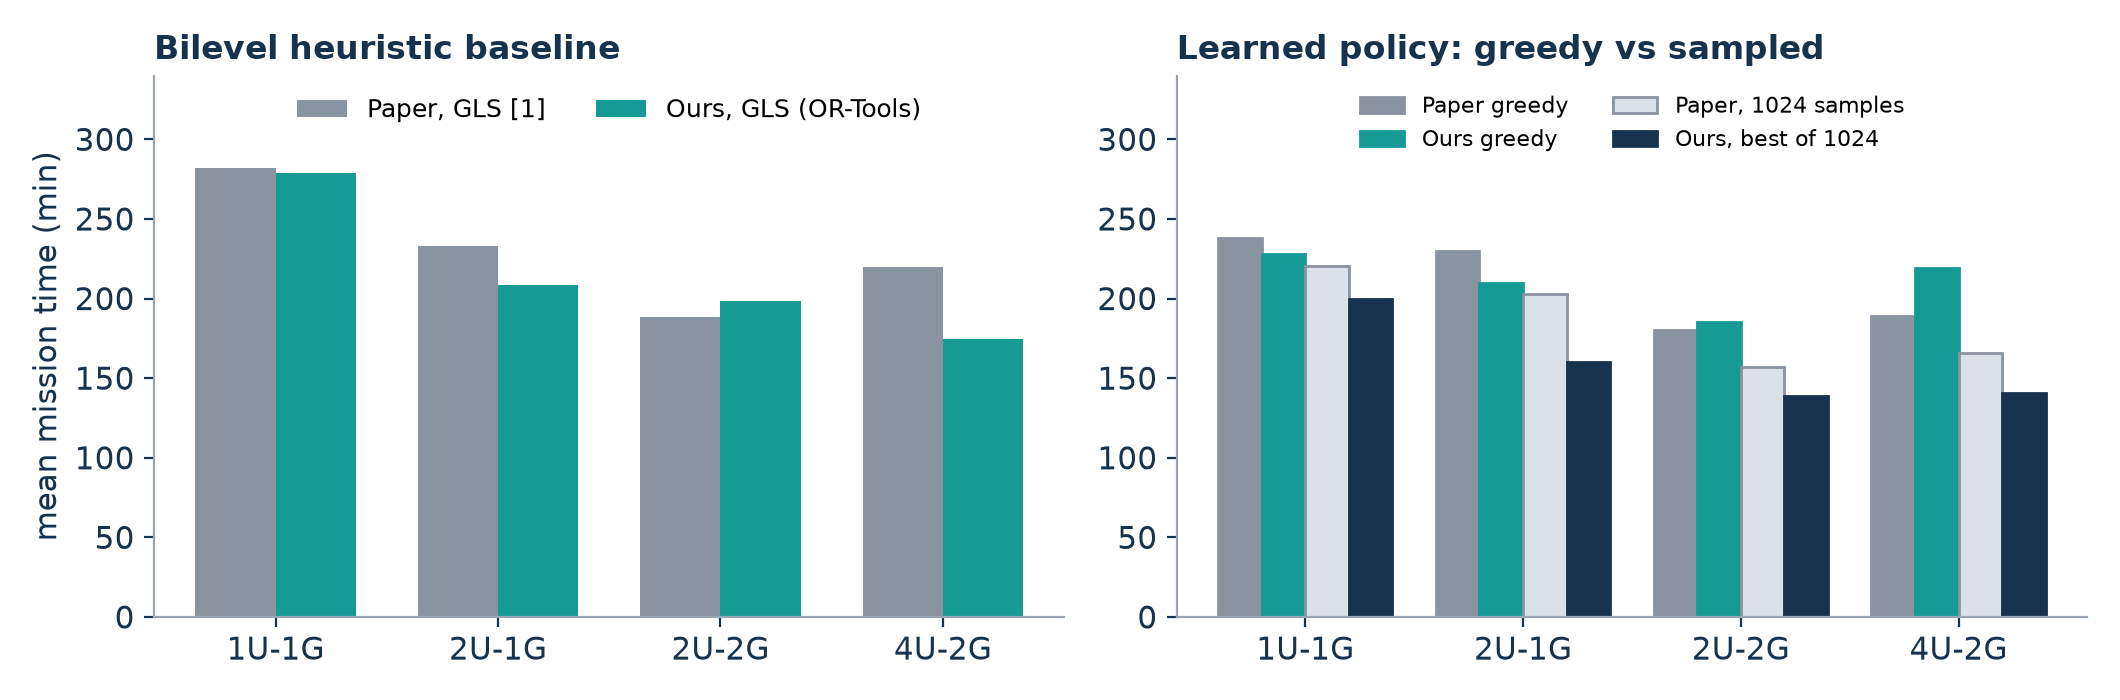
\includegraphics[width=0.97\linewidth]{assets/fig_baselines.png}\\[0.5mm]
{\small Our GLS / Tabu / SA baselines land in the paper's range. With 10{,}240 samples we reach 135 to 197\,min, below the paper's sampled results (reconstructed map, so not a claim to beat~\cite{base}).}
\end{frame}

\begin{frame}{6 \,Gazebo Test Bed: Do the Plans Hold Up in Physics?}
\centering
\begin{tikzpicture}[font=\scriptsize]
  \node[fgray, text width=2.3cm] (a) at (0,0) {Planned mission};
  \node[fb,    text width=2.3cm] (b) at (3.0,0) {World: roads, tasks, events};
  \node[fteal, text width=2.9cm] (c) at (6.2,0) {Wheeled UGV, flying UAV, lock-step replay};
  \node[famber,text width=2.9cm] (d) at (9.6,0) {Compare time, energy, UGV timing};
  \foreach \x/\y in {a/b,b/c,c/d} \draw[ar] (\x)--(\y);
\end{tikzpicture}\\[2mm]
\begin{columns}[T,onlytextwidth]
\begin{column}{0.47\textwidth}\centering
\fbox{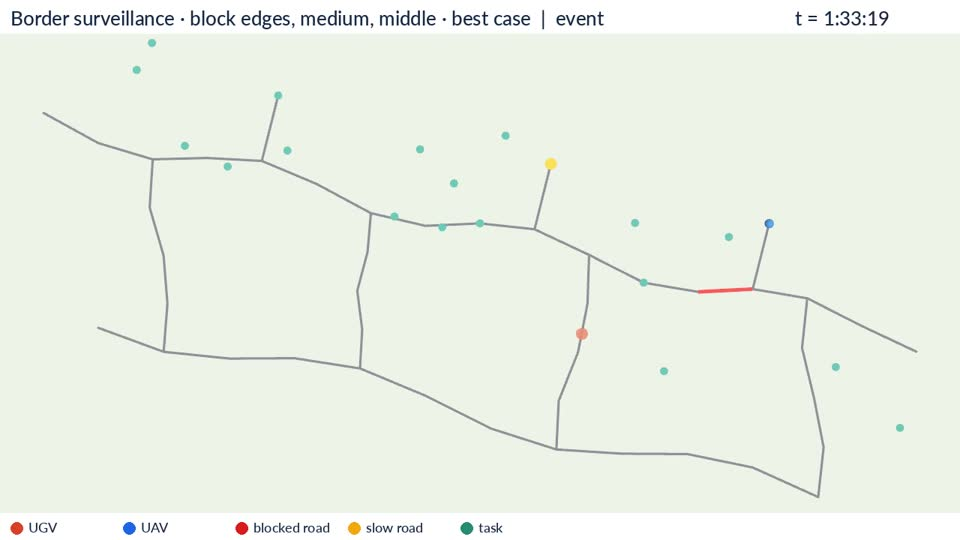
\includegraphics[width=\linewidth]{assets/flat_border_event.jpg}}\\[0.5mm]
{\scriptsize Flat ground, border map}
\end{column}
\begin{column}{0.47\textwidth}\centering
\fbox{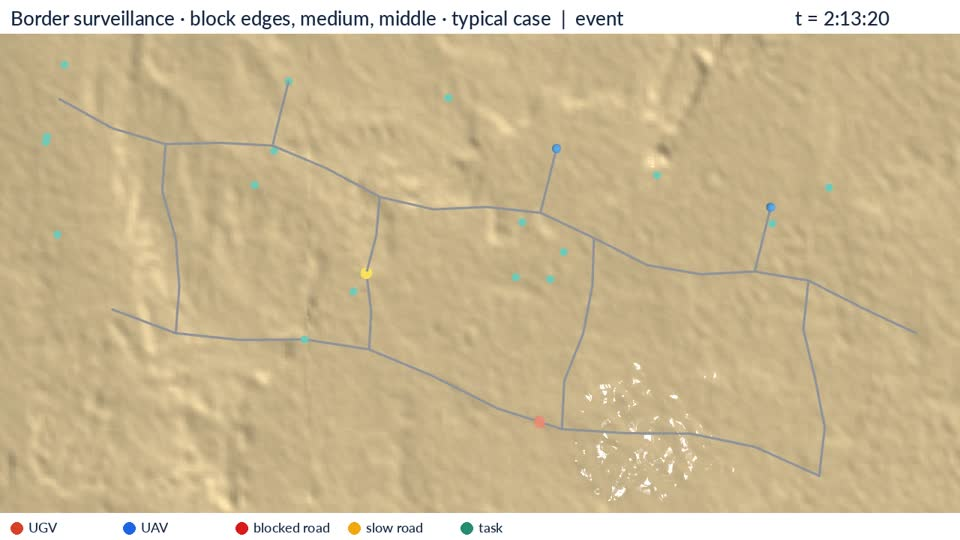
\includegraphics[width=\linewidth]{assets/terrain_border_event.jpg}}\\[0.5mm]
{\scriptsize Real terrain (open elevation data, 144\,m relief)}
\end{column}
\end{columns}
\vspace{1.5mm}
\begin{tikzpicture}\node[fteal, text width=12.3cm]{\textbf{22 replays} (16 flat, 6 terrain): mission time within \textbf{0.14\%} of the plan (at most 0.8\,min), UAV energy within 0.5\%, UGV arrives 11 to 16\,s late on average. This checks the plans; the learned policy is not run inside Gazebo~\cite{gazebo}.};\end{tikzpicture}
\end{frame}

\begin{frame}{6 \,Did the Hypotheses Hold?}
\centering\small
\renewcommand{\arraystretch}{1.5}
\begin{tabular}{@{}P{5.8cm}cP{5.4cm}@{}}
\toprule
\textbf{Hypothesis} & & \textbf{Evidence}\\
\midrule
H1 energy falls, time barely rises & \pmark & \xmark\ for routes (time and energy move together); \cmark\ for departure timing: $-$53 to $-$74\% energy, $+0$ min\\
H2 constrained beats fixed penalty & \xmark & A and B equal the control on all maps\\
H3 more disruption, more energy & \cmark & up to +29\% energy, early events worst\\
H4 same reliability, fewer replans & \cmark & same time, 1 to 3 fewer replans\\
\bottomrule
\end{tabular}\\[3mm]
{\small Failures appear only when a bridge is cut and the map is disconnected.}
\end{frame}

\begin{frame}{Conclusion and Limitations}
\begin{columns}[T,onlytextwidth]
\begin{column}{0.49\textwidth}
\begin{block}{What we showed}
\small
\begin{itemize}\setlength\itemsep{1.5mm}
\item Road events cost up to $+29\%$ energy; \textbf{event-triggered replanning} recovers it with few replans.
\item \textbf{Just-in-time departure}: $-53$ to $-74\%$ UAV energy at no cost in time.
\item With \textbf{sampling and a budget filter}: $-20\%$ time, $-65\%$ energy, budget met.
\item Gazebo reproduces the plans to within 0.14\% in time.
\end{itemize}
\end{block}
\end{column}
\begin{column}{0.49\textwidth}
\begin{block}{Limitations and next steps}
\small
\begin{itemize}\setlength\itemsep{1.5mm}
\item Learned energy-aware methods (A, B) do not beat the control.
\item 4U-2G policy 9 to 14\% slower than~\cite{base}; more training did not help, search does.
\item Replans only at recharge boundaries; one bad seed (fallback fixes the failures).
\item Gazebo replays plans only: run the policy and replanner inside it~\cite{gazebo}.
\end{itemize}
\end{block}
\end{column}
\end{columns}
\end{frame}

\begin{frame}{References}
\fontsize{5.7}{6.7}\selectfont\setlength{\itemsep}{0.5pt}
\begin{thebibliography}{99}
\bibitem{base} M. S. Mondal, S. Ramasamy, L. Russo, J. D. Humann, J. M. Dotterweich, and P. Bhounsule, ``How to coordinate UAVs and UGVs for efficient mission planning? Optimizing energy-constrained cooperative routing with a DRL framework,'' arXiv:2504.21111, 2025.
\bibitem{maini} P. Maini, K. Sundar, M. Singh, S. Rathinam, and P. B. Sujit, ``Cooperative aerial--ground vehicle route planning with fuel constraints for coverage applications,'' \emph{IEEE Trans. Aerosp. Electron. Syst.}, vol. 55, no. 6, pp. 3016--3028, 2019.
\bibitem{mrs} M. S. Mondal \emph{et al.}, ``Optimizing fuel-constrained UAV-UGV routes for large scale coverage: Bilevel planning in heterogeneous multi-agent systems,'' in \emph{Proc. Int. Symp. Multi-Robot Multi-Agent Syst. (MRS)}, 2023, pp. 114--120.
\bibitem{fan} M. Fan \emph{et al.}, ``Deep reinforcement learning for UAV routing in the presence of multiple charging stations,'' \emph{IEEE Trans. Veh. Technol.}, vol. 72, no. 5, pp. 5732--5746, 2023.
\bibitem{shi} G. Shi \emph{et al.}, ``Risk-aware UAV--UGV rendezvous with chance-constrained Markov decision process,'' in \emph{Proc. IEEE Conf. Decis. Control (CDC)}, 2022, pp. 180--187.
\bibitem{lin} X. Lin, Y. Yaz{\i}c{\i}o\u{g}lu, and D. Aksaray, ``Robust planning for persistent surveillance with energy-constrained UAVs and mobile charging stations,'' \emph{IEEE Robot. Autom. Lett.}, vol. 7, no. 2, pp. 4157--4164, 2022.
\bibitem{icra} M. S. Mondal \emph{et al.}, ``Risk-aware energy-constrained UAV--UGV cooperative routing using attention-guided reinforcement learning,'' in \emph{Proc. IEEE Int. Conf. Robot. Autom. (ICRA)}, 2025, pp. 13000--13006.
\bibitem{kool} W. Kool, H. van Hoof, and M. Welling, ``Attention, learn to solve routing problems!'' arXiv:1803.08475, 2018.
\bibitem{williams} R. J. Williams, ``Simple statistical gradient-following algorithms for connectionist reinforcement learning,'' \emph{Mach. Learn.}, vol. 8, pp. 229--256, 1992.
\bibitem{hurwitz} A. M. Hurwitz, J. M. Dotterweich, and T. A. Rocks, ``Mobile robot battery life estimation: Battery energy use of an unmanned ground vehicle,'' in \emph{Energy Harvesting and Storage: Materials, Devices, and Applications XI}, SPIE, vol. 11722, 2021, pp. 24--40.
\bibitem{gazebo} N. Koenig and A. Howard, ``Design and use paradigms for Gazebo, an open-source multi-robot simulator,'' in \emph{Proc. IEEE/RSJ Int. Conf. Intell. Robots Syst. (IROS)}, vol. 3, 2004, pp. 2149--2154.
\bibitem{code} M. S. Mondal \emph{et al.}, ``multi-uav-ugv-cooperative-routing-drl,'' source code, GitHub. [Online]. Available: \url{https://github.com/imsafwan/multi-uav-ugv-cooperative-routing-drl}
\end{thebibliography}
\end{frame}

\end{document}
